% ---
% JAVA EMBEDDED SUITE
%
% ---

% TODO
% - revisão do texto em .pdf

\chapter{Java Embedded Suite}

Este capítulo tem como objetivo demonstrar a plataforma \textit{Java Embedded}
- \textit{Java Embedded Suite} (\textit{JES}).

\section{Instalação}

A plataforma de prototipagem deve estar operacional com o sistema operacional
\textit{Linux} e a plataforma \textit{Java 8}, no caso de estudo a plataforma
\textit{Raspberry PI B+}. A figura \ref{fig:jes/configuracao} apresenta as
configurações do sistema em estudo.

\begin{figure}[H]
    \centering
    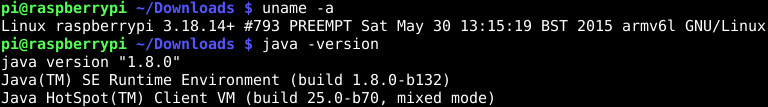
\includegraphics[width=0.7\linewidth]{figuras/java/configuracao}
    \caption{Configuração do Sistema}
    \label{fig:jes/configuracao}
\end{figure}

Para a plataforma de prototipagem é necessário a instalação do pacote
\textit{Oracle Java Embedded Suite 7.0}, necessário ter uma conta no site da
\textit{Oracle} para realizar o \textit{download}.

Transfira os arquivos \newline
\verb|jes-7.0-ga-bin-b11-linux-arm-runtime-15_nov_2012.zip|
 e \newline
\verb|jes-7.0-ga-b11-linux-samples-15_nov_2012.zip|
 do sistema operacional principal para o dispositivo remoto, basta
utilizar o comando \textit{SCP}:

\verb|scp </path/from/file> <user>@<address>:/path/to/destination|

Descompacte os arquivos, basta utilizar o comando \textit{UNZIP}:

\verb|unzip <file>|

O caminho para o \textit{JES} define a variável ambiente
\verb|$JES_HOME| no sistema. Os \textit{scripts} já definem as variáveis de
ambiente necessárias para o sistema executar cada tipo de aplicação do pacote
\textit{JES}.

\subsection{Pacote Oracle Java Embedded Suite ZIP}

O pacote \textit{Oracle Java Embedded Suite ZIP} consiste de cinco diretórios:

\begin{itemize}

    \item \textit{glassfish}: este diretório contém servidor de aplicações
    \textit{GlashFish} através da biblioteca \verb|glassfish-jes.jar|;

    \item \textit{javadb}: este diretório contém o banco de dados
    \textit{Derby} através das bibliotecas \verb|derby.jar| e
    \verb|derbytools.jar|;

    \item \textit{jersey}: este diretório contém o \textit{framework} de
    aplicações \textit{Jersey};

    \item \textit{jre}: este diretório contém o \textit{runtime} para a
    execução de aplicações \textit{Java}. Não é necessário, quando o
    \textit{Java 8} encontrasse corretamente instalado;

    \item \textit{samples}: este diretório contém exemplos de aplicações e os
    \textit{scripts} para a execução das aplicações.

\end{itemize}

O arquivo \verb|jes-verify.sh| realiza o diagnóstico da instalação do ambiente
de execução.

\subsection{Desenvolvimento}

O processo de desenvolvimento não difere da forma utilizada em servidores
tradicionais através de aplicações \textit{Web application}, em codificar e
realizar a implantação da aplicação.

O exemplo implementa uma aplicação \textit{Web} para a monitoração de
temperatura da Unidade de Processamento Gráfico - \textit{Graphics Processing
  Unit} (\textit{GPU}) do \textit{Raspberry PI} através do comando
\verb|/opt/vc/bin/vcgencmd measure_temp| do sistema operacional.

\subsubsection{Codificação}

A aplicação consiste de um \textit{software} \textit{Servlet} com a definição
do método \verb|doGet()|, sendo o código final apresentado abaixo:

\begin{verbatim}
// MonitorTemp.java
package ufabc;

import java.io.BufferedReader;
import java.io.IOException;
import java.io.InputStreamReader;
import javax.servlet.ServletException;
import javax.servlet.annotation.WebServlet;
import javax.servlet.http.HttpServlet;
import javax.servlet.http.HttpServletRequest;
import javax.servlet.http.HttpServletResponse;

@WebServlet(urlPatterns = {"/"})
public class MonitorTemp extends HttpServlet {

    @Override
    protected void doGet(HttpServletRequest request,
            HttpServletResponse response)
            throws ServletException, IOException {
        response.getWriter().write("<b>Monitoração da GPU<b><br/>");
        Runtime runtime = Runtime.getRuntime();
        BufferedReader br = new BufferedReader(
                new InputStreamReader(
                        runtime.exec("/opt/vc/bin/vcgencmd measure_temp")
                        .getInputStream()));
        response.getWriter().write(br.readLine());
    }
}
\end{verbatim}

\subsubsection{Implantação}

A implantação da aplicação é por transferir o arquivo para o dispositivo remoto
e executar via o \textit{script} para o tipo de aplicação:

\begin{itemize}

    \item \verb|gfhost.sh|: utilizado para implantar a aplicação \textit{Web}
    no \textit{JES}, permite múltiplas aplicações ao mesmo tempo;

    \item \verb|hclient.sh|: utilizado para acessar serviços \textit{Web} -
    \textit{Web services};

    \item \verb|hstorage.sh|: utilizado para aplicação com o \textit{Java DB};

    \item \verb|lwhost.sh|: utilizado para implantar a aplicação de serviço
      \textit{Web} \textit{Web service} no \textit{JES}.

\end{itemize}

O \textit{script} \verb|config.sh| permite a configuração do \textit{classpath}
e dos argumentos passados para o \textit{runtime} do \textit{Java}.

Para realizar a implantação do exemplo, basta utilizar o \textit{script}
\verb|gfhost.sh| no caminho \verb|$JES_HOME/samples/dist/run|:

\verb|./gfhost.sh ../../../dist/MonitorTemp.war|

Ao final da implantação será exibida a mensagem apresentada na figura
\ref{fig:java-me/java-jes-deploy}.

\begin{figure}[H]
    \centering
    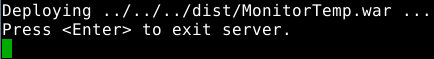
\includegraphics[width=0.7\linewidth]{figuras/java/java-jes-deploy.png}
    \caption{Implantação da Aplicação}
    \label{fig:java-me/java-jes-deploy}
\end{figure}

No navegador basta acessar o endereço do \textit{Raspberry PI} pela porta
\verb|8080| e adicionar o caminho da aplicação, conforme apresentado na figura
\ref{fig:java-me/java-jes-browser}.

\begin{figure}[H]
    \centering
    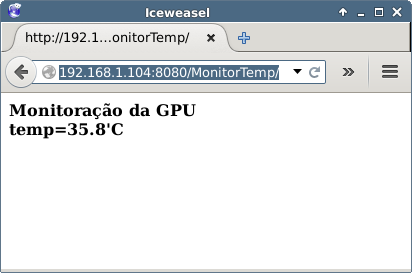
\includegraphics[width=0.7\linewidth]{figuras/java/java-jes-browser.png}
    \caption{Monitor de Temperatura da GPU}
    \label{fig:java-me/java-jes-browser}
\end{figure}

\section{Aplicações para a Internet das Coisas}

Um servidor de aplicações traz a \textit{Internet} das Coisas -
\textit{Internet of Things} (\textit{IoT}) uma interface para a
disponibilização de serviços, seja para a comunicação com usuários quanto
outros dispositivos embarcados. O \textit{JES} permite a interoperabilidade com
aplicações \textit{Java ME Embedded}, trazendo o poder dos periféricos de baixo
nível como fonte de dados. Esses serviços agrega as possibilidades de obtenção,
armazenamento e processamento de dados.

\newpage
\section{Resultados}

Os resultados demonstram a visão na qual a plataforma \textit{JES} contribui
para o desenvolvimento de aplicações destinadas a \textit{IoT}.

\subsection{Positivos}

\begin{itemize}

    \item A possibilidade de implantar um servidor de aplicações \textit{Web},
    banco de dados e \textit{Web services} em um sistema embarcado;

    \item Interfaceamento com as classes de aplicações \textit{Java ME
    Embedded}.

\end{itemize}

\subsection{Negativos}

\begin{itemize}

    \item Não possui muitos componentes para os servidores, assim reduzindo as
    possibilidades de desenvolvimento.

\end{itemize}
